\documentclass[12pt,italian]{report}
\usepackage{tesi}
\usepackage{algorithm}
\usepackage{algorithmic}
%\usepackage[section]{placeins}

%
%			INFORMAZIONI SULLA TESI
%			DA COMPILARE!
%

% CORSO DI LAUREA:
\def\myCDL{Corso di Laurea magistrale in\\Informatica}
% TITOLO TESI:
\def\myTitle{Il titolo\\della tesi}

% AUTORE:
\def\myName{Lorenzo D'Alessandro}
\def\myMat{Matr. Nr. 939416}

% RELATORE E CORRELATORE:
\def\myRefereeA{Relatore 1}
\def\myRefereeB{Correlatore 1}

% ANNO ACCADEMICO
\def\myYY{2020-2021}

% Il seguente comando introduce un elenco delle figure dopo l'indice (facoltativo)
%\figurespagetrue

% Il seguente comando introduce un elenco delle tabelle dopo l'indice (facoltativo)
%\tablespagetrue

%
%			PREAMBOLO
%			Inserire qui eventuali package da includere o definizioni di comandi personalizzati
%

% Package di formato
\usepackage[a4paper]{geometry}		% Formato del foglio
\usepackage[italian]{babel}			% Supporto per l'italiano
\usepackage[utf8]{inputenc}			% Supporto per UTF-8
%\usepackage[a-1b]{pdfx}			% File conforme allo standard PDF-A (obbligatorio per la consegna)

% Package per la grafica
\usepackage{graphicx}				% Funzioni avanzate per le immagini
\usepackage{hologo}					% Bibtex logo with \hologo{BibTeX}
%\usepackage{epsfig}				% Permette immagini in EPS
%\usepackage{xcolor}				% Gestione avanzata dei colori

% Package tipografici
\usepackage{amssymb,amsmath,amsthm} % Simboli matematici
\usepackage{listings}				% Scrittura di codice

% Package ipertesto
\usepackage{url}					% Visualizza e rendere interattii gli URL
\usepackage{hyperref}				% Rende interattivi i collegamenti interni


\begin{document}

% Creazione automatica del frontespizio
\frontespizio
\beforepreface

% 
%			PAGINA DI DEDICA E/O CITAZIONE
%			facoltativa, questa è l'unica cosa che dovete formattare a mano, un po' come vi pare
%

{\raggedleft \large \sl Dedica \\}
         
% 
%			PREFAZIONE (facoltativa)
%

%\prefacesection{Prefazione}
%Le prefazioni non sono molto comuni, tuttavia a volte capita che qualcuno voglia dire qualcosa che esuli dal lavoro in s\'e (come un meta-commento sull'elaborato), o voglia fornire informazioni riguardanti l'eventuale progetto entro cui la tesi si colloca (in questo caso \`e probabile che sia il relatore a scrivere questa parte).

%
%			RINGRAZIAMENTI (facoltativi)
%

\prefacesection{Ringraziamenti}
Questa sezione, facoltativa, contiene i ringraziamenti.

%
%			Creazione automatica dell'indice
%

\afterpreface

% 
%			CAPITOLO 1: Introduzione o Abstract
% 

\chapter{Introduzione}
\label{cap:introduzione}

Introduzione...

\section{I contenuti}
\label{sec:contenuti}

Spiegazione problema...


\section{Organizzazione della tesi}
\label{sec:organizzazione}

Organizzazione tesi...

% 
%			CAPITOLO 2: Stato dell'arte
% 



\chapter{Stato dell'arte}
\label{chap:stato_arte}
I recommender system (RS) sono algoritmi mirati a generare consigli significativi a un insieme di utenti per articoli o prodotti che potrebbero interessarli \cite{recsys-definition}. La definizione di oggetto è generica e include ad esempio film da guardare, libri da leggere, prodotti da comprare, punti di interesse, etc. 
Quando gli utenti interagiscono con il sistema generano dei feedback. Questi feedback possono essere di due tipi: espliciti o impliciti. I feedback espliciti sono valori numerici che un utente assegna ad un prodotto, i feedback impliciti riflettono indirettamente le opinioni di un utente osservando la cronologia degli acquisti, i link aperti, gli elementi visualizzati, etc.
Basandosi sui feedback passati, i sistemi di raccomandazione imparano un modello per prevedere quanto un utente può essere interessato a nuovi oggetti. Questi oggetti sono poi ordinati in base alla pertinenza prevista per l'utente. In ultimo, gli oggetti con il rank più alto vengono suggeriti all'utente. La relazione tra utenti e oggetti è rappresentata con una matrice $R_M$ in cui sono memorizzati i rating passati degli utenti.
La \textit{ratings matrix} è definita come: 
$$
R_M: U \times I \rightarrow R
$$
dove $U = \{u_1, \dots, u_m\}$ rappresenta l'insieme degli utenti, $I = \{i_1,\dots, i_n\}$ rappresenta l'insieme degli utenti, e $R = \{r_1, \dots, r_k\}$ rappresenta l'insieme dei possibili ratings che un utente ha espresso riguardo a degli oggetti \cite{survey-mattia}. Un valore mancante nella ratings matrix può avere due significati: l'utente non vuole esprimere un'opinione su un oggetto specifico, oppure l'utente non conoscendo ancora l'oggetto non può averlo valutato.

\vspace{5mm}
\noindent I recommender system si dividono principalmente in tre categorie:
\begin{itemize}
	\item collaborative filtering
	\item content-based
	\item hybrid
\end{itemize}

\noindent In figura \autoref{fig:cb-cf} è schematizzato il modo diverso in cui operano i metodi collaborative filtering rispetto a quelli content-based.

\begin{figure}
  \includegraphics[width=\linewidth]{immagini/cb_cf_schema.png}
  \caption{Collaborative filtering vs Content-based}
  \label{fig:cb-cf}
\end{figure}

\section{Collaborative filtering recommender system}
Collaborative filtering (CF) è la tecnica di raccomandazione più popolare e ampiamente utilizzata nei RS. Il presupposto alla base di CF è che le persone con preferenze simili valuteranno gli stessi oggetti con ratings simili. CF quindi sfrutta le informazioni sul comportamento passato o le opinioni di una comunità di utenti esistente per prevedere quali elementi potranno piacere o saranno interessanti per l'utente corrente del sistema \cite{recsys-intro}. Gli approcci CF puri non sfruttano né richiedono alcuna conoscenza degli oggetti stessi ma solo dei feedback degli utenti. La classe di algoritmi più famosa è quella di Matrix Factorization, ma recentemente sono stati sviluppati diversi approcci basati sul deep learning \cite{deep-learning-survey}.

\subsection{Vantaggi e svantaggi} \label{ssec:pros-cons-cf}
\textbf{Vantaggi:}
\begin{itemize}

 \item \textit{Nessuna conoscenza del dominio necessaria:} il modello può funzionare in domini in cui non c'è molto contenuto associato agli oggetti e in cui il contenuto è difficile da analizzare per un sistema informatico (come opinioni e ideali) \cite{recsys-principle-methods-evaluation}.
 
 \item \textit{Serendipity:} il modello ha la capacità di fornire consigli fortuiti, il che significa che può consigliare elementi pertinenti per l'utente anche senza che il contenuto si trovi nel profilo dell'utente permettendo all'utente di scoprire nuovi interessi \cite{recsys-principle-methods-evaluation} \cite{cf-advantages-google}.
\end{itemize}

\noindent \textbf{Svantaggi:}
\begin{itemize}
 \item \textit{Problema del cold-start:} Si riferisce alla situazione in cui il sistema di raccomandazione non ha abbastanza informazioni su un utente od un oggetto per poter fare previsioni rilevanti. Un nuovo oggetto inserito nel RS di solito non ha voti, ed è quindi improbabile che venga raccomandato. Un oggetto non consigliato passa inosservato a gran parte della community. Il problema è presente anche per i nuovi utenti: gli utenti che hanno espresso nessuna o poche valutazioni non ricevono raccomandazioni affidabili \cite{cold-start}.   
 
 \item  \textit{Problema di data sparsity:} questo è il problema che si verifica a causa della mancanza di informazioni sufficienti, cioè quando solo pochi rispetto al numero totale di oggetti disponibili in un database sono valutati dagli utenti. Ciò porta ad una rating matrix sparsa, e raccomandazioni poco efficaci \cite{recsys-principle-methods-evaluation}.
 
 \item \textit{Scalabilità:} Questo è un altro problema associato agli algoritmi di raccomandazione perchè il tempo di computazione cresce linearmente con il numero di utenti e oggetti. Un sistema di raccomandazione efficiente con un dataset limitato potrebbe non esserlo con un dataset di dimensioni maggiori \cite{recsys-principle-methods-evaluation}.
\end{itemize}

\subsection{Matrix factorization} \label{ssec:mf}
Gli algoritmi basati su matrix factorization (MF) caratterizzano sia utenti che oggetti mediante dei vettori di fattori estratti dai pattern sui ratings. Una corrispondenza alta tra i fattori di un utente e un oggetto porta ad una raccomandazione. Questi metodi sono diventati popolari negli ultimi anni perchè combinano scalabilità e accuratezza.

Più formalmente, i modelli basati su matrix factorization mappano utenti e oggetti in uno spazio di fattori latenti di dimensionalità $f$, tale che le interazioni tra utenti e oggetti sono modellate come prodotti in quello spazio. Di conseguenza, ogni oggetto $i$ è associato con un vettore $q_i \in \mathbb{R}^f$, e ogni utente $u$ con un vettore $p_u \in \mathbb{R}^f$. Per un dato oggetto $i$, gli elementi di $q_i$ indicano la misura in cui l'oggetto possiede quei fattori, positivi o negativi. Per un dato utente $u$, gli elementi di $p_u$ indicato l'entità dell'interesse che l'utente ha per gli oggetti che hanno un valore alto sui fattori corrispondenti, positivi o negativi. Il prodotto scalare $q_i^Tp_u$ indica l'interesse dell'utente $u$ per le caratteristiche dell'oggetto $i$ \cite{matrix-factorization}. Quindi il rating $r_{ui}$ può essere approssimato come

\begin{equation} \label{eq:dot_product}
r_{ui} = q_i^Tp_u
\end{equation}
Il problema principale è calcolare il mapping di ogni oggetto e utente in dei vettori $q_i, p_u \in \mathbb{R}^f$. Una volta che il recommender system ha completato il mapping, può facilmente stimare il rating che un utente darà a qualsiasi oggetto utilizzando l'equazione \ref{eq:dot_product}. 

In \autoref{fig:matrix_factorization} è mostrato come la matrice dei ratings $A \in \mathbb{R}^{m \times n}$, con $m$ numero di utenti e $n$ numero di oggetti, viene decomposta in due matrici di dimensionalità minore:

\begin{itemize}
	\item Una matrice di embedding per gli utenti $P \in \mathbb{R}^{m \times f}$, in cui la riga $i$ è l'embedding dell'utente $i$
	\item Una matrice di embedding per gli oggetti $Q \in \mathbb{R}^{n \times f}$, in cui la riga $j$ è l'embedding dell'oggetto $j$
\end{itemize}
Gli embedding di $P$ e $Q$ sono imparati in modo tale che il prodotto $PQ^T$ sia una buona approssimazione della matrice dei ratings $A$ \cite{mf-google}.

\begin{figure}
  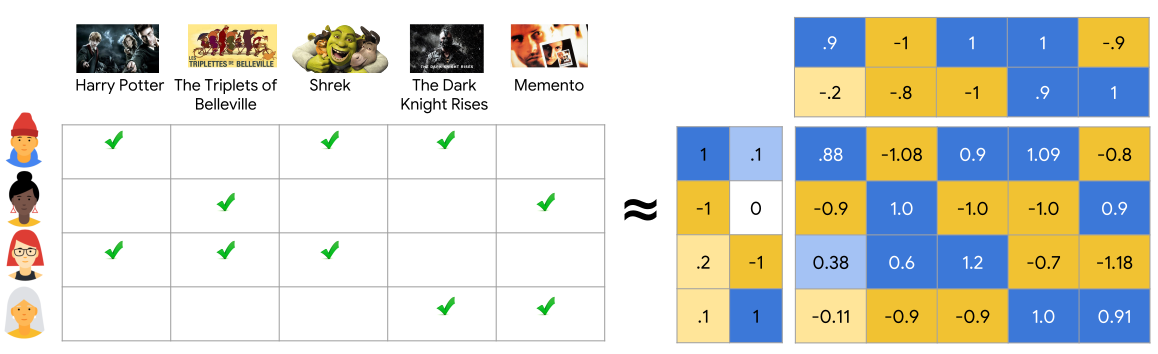
\includegraphics[width=\linewidth]{immagini/matrix_factorization.pdf}
  \caption{Approssimazione matrice dei ratings con matrix factorization}
  \label{fig:matrix_factorization}
\end{figure}

\section{Content-based recommender system}
Nei recommender system content-based (CB), gli attributi descrittivi degli oggetti sono usati per produrre raccomandazioni. Il termine "content" indica queste descrizioni. Nei metodi content-based i ratings degli utenti sono combinati con le informazioni disponibili sugli oggetti, per poi essere usati come training data per creare un modello di classificazione o regressione specifico per l'utente. Questo modello specifico per l'utente viene utilizzato per prevedere se alla persona corrispondente piacerà un articolo per il quale la sua valutazione è ancora sconosciuta \cite{recsys-book}.

Mentre nei CF la similarità tra due oggetti (o due utenti) è calcolato come la correlazione o la similarità tra i ratings forniti dagli altri utenti, i recommender system content-based sono progettati per consigliare oggetti simili a quelli che l'utente ha preferito in passato. Non considerando gli altri utenti, la lista di raccomandazioni può essere generata anche se c'è un solo utente nel sistema.

\subsection{Vantaggi e svantaggi}
\textbf{Vantaggi:}
\begin{itemize}
 \item \textit{Consigliare nuovi oggetti:} Questi modelli hanno la capacità di consigliare nuovi oggetti anche se non ci sono valutazioni fornite dagli utenti a differenza dei modelli collaborative filtering \cite{recsys-principle-methods-evaluation}.
 
 \item \textit{Trasparenza:} Le spiegazioni su come funziona il sistema di raccomandazione possono essere fornite elencando esplicitamente le caratteristiche del contenuto che hanno causato la presenza di un oggetto nell'elenco delle raccomandazioni \cite{transparency}. 
\end{itemize}

\noindent \textbf{Svantaggi:}
\begin{itemize}
 \item \textit{Features degli oggetti:} la precisione del modello dipende dall'insieme delle features che descrivono gli oggetti. Identificare le features più rilevanti non è semplice e dipende molto dall'applicazione specifica \cite{survey-mattia}.
 
 \item \textit{Content overspecialization:} Dato che i metodi CB si affidano solo alle caratteristiche degli oggetti già valutati dall'utente corrente, egli riceverà solo raccomandazioni simili ad altri oggetti già definiti nel suo profilo \cite{recsys-principle-methods-evaluation}.
 
 \item \textit{Dimensione training set:} In modo da consentire a un RS content-based di imparare le preferenze di un utente, egli dovrà valutare un numero sufficiente di oggetti. In caso contrario, il RS non avrà sufficienti informazioni per imparare un modello accurato e fallirà nel raccomandare oggetti a utenti con pochi o nessun ratings.
\end{itemize}

\section{Hybrid recommender system}
I modelli ibridi combinano tipi diversi di sistemi di raccomandazione per formare dei modelli in grado di superare le debolezze dei modelli singoli. In \cite{recsys-book} sono descritti tre modi per creare recommender system ibridi:

\begin{enumerate}
 \item \textit{Ensemble design:} Con questo metodo i risultati degli algoritmi base sono combinati in un output singolo più robusto. Il principio fondamentale è molto simile ai metodi di ensemble usati in molte applicazioni di data mining come clustering, classificazione e analisi degli outlier. 
Gli ensemble design possono essere formalizzati nel modo seguente. Sia $R^k$ una matrice $m \times n$ contenente le predizioni di $m$ utenti per $n$ oggetti dell'algoritmo $k$-esimo, con $k \in \{1, \dots ,q\}$. Pertanto, un totale di $q$ algoritmi diversi sono usati per ottenere queste predizioni. L'elemento $(u,j)$-esimo di $R^k$ contiene il rating predetto per l'utente $u$ sull'oggetto $j$ dall'algoritmo $k$-esimo. Gli elementi della matrice originale $R$ sono replicati in ogni $R^k$, e solo gli elementi non presenti in $R$ variano nei differenti $R^k$ a causa dei diversi risultati degli algoritmi. Il risultato finale è ottenuto combinando le predizioni $R^1, \dots, R^q$ in un singolo output. La combinazione può essere fatta in vari modi, ad esempio calcolando la media pesata delle varie predizioni. Le caratteristiche comuni di questi algoritmi sono usare sistemi di raccomandazione già esistenti e produrre uno score/ranking unico.
 \item \textit{Monolithic design:} In questo caso, viene creato un algoritmo di raccomandazione integrato utilizzando vari tipi di dati. A volte non esiste una chiara distinzione tra le varie parti (es. content-based e collaborative filtering) dell'algoritmo. In altri casi, potrebbe essere necessario modificare gli algoritmi algoritmi di raccomandazione esistenti per essere usati all'interno dell'approccio generale, anche quando c'è una chiara distinzione tra gli algoritmi utilizzati.  Pertanto, questo approccio tende a integrare più strettamente le varie fonti di dati e non è possibile visualizzare facilmente i singoli componenti come black-boxes separate.
 \item \textit{Mixed systems:}  Come per gli ensembles, questi sistemi usano diversi algoritmi di raccomandazione come black-boxes, ma gli oggetti raccomandati dai vari sistemi sono presentati insieme senza essere combinati.
\end{enumerate} 

\section{Context-aware recommender system}
I recommender system context-aware (CARS) producono le loro raccomandazioni utilizzando informazioni addizionali che definiscono la situazione di un utente. Queste informazioni addizionali sono chiamate \textit{contesto}.

\noindent Alcuni esempi di contesto sono:
\begin{enumerate}
 \item \textit{Data e ora:} Dalle informazioni di data e ora è possibile estrarre diverse features contestuali come il momento della giornata, il giorno della settimana, week-end, vacanze, stagioni ed altro ancora. Una raccomandazione potrebbe essere rilevante la mattina ma non il pomeriggio, e viceversa. Le raccomandazioni sui vestiti invernali o estivi possono essere molto diverse.
 \item \textit{Posizione:} Con la crescente popolarità del GPS disponibile ormai su qualunque telefono, le raccomandazioni sensibili alla posizione dell'utente hanno guadagnato importanza. Per esempio, un viaggiatore potrebbe desiderare raccomandazioni su ristoranti vicini alla propria posizione. Questo può essere fatto aggiungendo la posizione come contesto nel recommender system.
 \item \textit{Informazioni sociali:} Il contesto sociale è spesso importante per un sistema di raccomandazione. Le informazioni su amici, tag e cerchie sociali di un utente possono avere un impatto sul processo di raccomandazione. Per esempio una ragazzo potrebbe scegliere di guardare un film diverso a seconda che lo guardi con i suoi genitori o con i suoi amici.
\end{enumerate} 

\noindent Il contesto può essere ottenuto in vari modi \cite{recsys-handbook} che includono:
\begin{enumerate}
 \item \textit{Esplicitamente} ponendo domande dirette alle persone rilevanti o richiedendo le informazioni con altri mezzi. Per esempio, un sito web potrebbe ottenere informazioni contestuali chiedendo agli utenti di compilare un form.
 \item \textit{Implicitamente} dai dati o dall'ambiente, come il cambio di posizione rilevato da una compagnia di telefonia mobile. In questo caso non è necessario fare nulla in termini di interazione con l'utente o altre fonti di informazioni contestuali perché l'informazione contestuale è acceduta direttamente e i dati sono estratti da essa.
 \item \textit{Per inferenza} usando metodi statistici o di data mining. 
\end{enumerate}

\subsection{Approccio multidimensionale}
Il problema tradizionale di raccomandazione può essere visto come apprendere una funzione che associa le coppie utente-oggetto ai ratings. La funzione corrispondente $f_R$ è definita come:

$$
f_R : U \times I \rightarrow rating
$$
Quindi la rating function mappa da uno spazio bidimensionale di utenti e oggetti ai ratings.
I CARS generalizzano questo metodo utilizzando un approccio multidimensionale in cui la rating function può essere vista come un mapping da una matrice $n$-dimensionale all'insieme dei ratings \cite{survey-mattia}.
$$
f_R : D_1 \times D_2 \dots \times D_n \rightarrow rating
$$
In questo caso, il risultato è un cubo n-dimensionale al posto che una matrice bidimensionale. Le diverse dimensioni sono denotate come $D_1 \dots D_n$. Due di queste dimensioni saranno sempre utenti e oggetti, le altre $D_i$ dimensioni corrispondono alle features del contesto \cite{recsys-book}. In \autoref{fig:ratings-cube} è mostrato un esempio di un cubo tridimensionale che memorizza i ratings per $User \times Items \times Location$, in cui $f_R(u_1, i_4, home) = 5$ significa che l'utente $u_1$ ha valutato con un punteggio pari a 5 l'oggetto $i_4$ mentre era a casa.

Il contesto può essere applicato nelle varie fasi del processo di raccomandazione. Come rappresentato in \autoref{fig:context-paradigm} si possono identificare tre paradigmi principali per integrare il contesto nei sistemi di raccomandazione \cite{recsys-handbook}:

\begin{figure}
  \centering
  \includegraphics[scale=0.80]{immagini/rating_cube.png}
  \caption{Esempio di un cubo multidimensionale per $User \times Item \times Location$}
  \label{fig:ratings-cube}
\end{figure}

\begin{enumerate}
 \item \textit{Contextual pre-filtering:} In questo paradigma, le informazioni riguardo il contesto attuale sono utilizzate per selezionare o costruire l'insieme dei dati rilevanti (la matrice dei ratings). Poi i ratings mancanti dai dati selezionati possono essere predetti utilizzando qualsiasi sistema di raccomandazione 2D tradizionale.
 \item \textit{Contextual post-filtering:} In questo paradigma, le informazioni contestuali sono inizialmente ignorate e i ratings sono predetti utilizzando qualsiasi sistema di raccomandazione 2D tradizionale. Poi, l'insieme di raccomandazioni non rilevanti nel contesto $c$ sono filtrate, e la lista di raccomandazioni è regolata in base a $c$.
 \item  \textit{Contextual modeling:} Mentre gli approcci di contextual pre-filtering e post filterning fanno uso di una funzione di raccomandazione 2D, gli approcci di contextual modeling danno luogo a funzioni di raccomandazione veramente multidimensionali che rappresentano modelli predittivi o euristiche che incorporano informazioni contestuali in aggiunta ai dati di utenti e oggetti.
\end{enumerate}

\begin{figure}
  \includegraphics[width=\linewidth]{immagini/paradigm_for_context_inclusion.png}
  \caption{Paradigmi per incorporare il contesto nei sistemi di raccomandazione}
  \label{fig:context-paradigm}
\end{figure}

\section{Alternating least square}
Alternating least square (ALS) \cite{als} è un algoritmo di matrix factorization stato dell'arte per quanto riguarda i feedback impliciti. ALS è un processo di ottimizzazione iterativo in cui ad ogni iterazione si cerca di arrivare il più vicino possibile a una rappresentazione fattorizzata dei dati originali \cite{als-medium}. 

\subsection{Feedback impliciti}
I feedback impliciti hanno alcune importanti caratteristiche che li distinguono dai feedback espliciti e impediscono di usare direttamente algoritmi progettati con i feedback espliciti in mente \cite{als}:
\begin{enumerate}
 \item \textit{Non ci sono feedback negativi.} Osservando il comportamento di un utente, è possibile inferire quali oggetti gli interessano e che quindi ha scelto di consumare. \'E difficile però capire in modo affidabile quali oggetti l'utente non apprezza. Per esempio, un utente che non ha guardato una serie tv potrebbe non averlo fatto perchè non interessato a quella serie, oppure perché non la conosceva. Questa asimmetria non esiste nei feedback espliciti in cui un utente si esprime su cosa gli piace e cosa non gli piace. Anche i dati mancanti sono un problema, nei feedback espliciti si conosce quali ratings non sono stati espressi dall'utente, nei feedback impliciti no.
 
 \item \textit{I feedback impliciti sono intrinsicamente rumorosi.} Tenendo traccia passivamente dei comportamenti degli utenti è difficile distinguere il caso in cui un utente ha consumato un oggetto perchè davvero interessato o per altri motivi.
 
 \item Il valore numerico dei feedback espliciti indica la \textit{preferenza}, mentre il valore numerico dei feedback impliciti indica la \textit{confidenza}. I sistemi basati sui feedback espliciti permettono all'utente di impostare il loro livello di preferenza su un oggetto, ad esempio con un voto da 1 a 5. I feedback impliciti invece descrivono la frequenza di un'azione, ma un valore più alto  non indica per forza una preferenza maggiore
\end{enumerate}

\subsection{Il modello}
Per prima cosa vanno formalizzati i concetti di preferenza e confidenza. La preferenza di un utente $u$ per un item $i$ è indicata con un valore binario $p_{ui}$:
$$
p_{ui} =     \begin{cases}
				1 \;\;\; r_{ui} > 0 \\
				0 \;\;\; r_{ui} = 0
              \end{cases}
$$
In pratica, se un utente $u$ ha consumato un oggetto $i$ ($r_{ui} > 0$), allora si ha un indicazione che $u$ è interessato a $i$. Diversamente, se $u$ non ha mai consumato $i$ la preferenza è uguale a 0. Inoltre, con l'aumento del valore di $r_{ui}$ si ha un indicazione più forte che l'utente sia davvero interessato all'oggetto. Di conseguenza, si può indicare con $c_{ui}$ la confidenza nell'osservare $p_{ui}$. Una possibile scelta è
$$
c_{ui} = 1 + \alpha r_{ui}
$$
In questo modo, si ha una confidenza minima su $p_{ui}$ per ogni coppia utente-oggetto, ma osservando più preferenze positive la confidenza su $p_{ui} = 1$ aumenta. La velocità di incremento è controllata dalla costante $\alpha$

Come spiegato nella \autoref{ssec:mf}, l'obbiettivo è trovare un vettore $x_u \in R^f$ per ogni utente $u$, ed un vettore $y_i \in R^f$ per ogni oggetto $i$ che fattorizzano le preferenze degli utenti. Le preferenze possono essere poi calcolate come $p_{ui} = x_u^Ty_i$. I vettori latenti in ALS sono calcolati minimizzando la funzione obbiettivo:	
$$
\min_{x_*,y_*} \sum_{u,i} c_{ui} (p_{ui} - x_u^Ty_i)^2 + 
\lambda \left( \sum_u ||x_u||^2 + \sum_i ||y_i||^2 \right)
$$
Il termine $\lambda \left( \sum_u ||x_u||^2 + \sum_i ||y_i||^2 \right)$ è necessario per regolarizzare il modello ed evitare l'overfitting durante il training. Il valore esatto di $\lambda$ dipende dai dati e si determina tramite cross validation. 
Quando il vettore latente degli utenti o degli oggetti rimane fissato, la funzione obbiettivo diventa quadratica è si può calcolare un minimo globale. Questo porta ad un processo di ottimizzazione con il metodo dei minimi quadrati, in cui si alterna tra il ricalcolare il vettore degli utenti mantenendo fissato quello degli oggetti e viceversa. Ad ogni step il valore della funzione di costo diminuisce.

\section{Neural collaborative filtering} \label{sec:ncf}
Gli algoritmi basati su matrix factorization sono sicuramente i più popolari nell'ambito dei sistemi di raccomandazione collaborative filtering. Nonostante l'efficacia di questi modelli, le loro performance  posso variare in base alla scelta della funzione di interazione. Ad esempio, per quanto riguarda il task di rating prediction su feedback espliciti, è noto che le performance di MF possono essere migliorate incorporando il bias di utenti e oggetti nella funzione di interazione. Anche se si tratta solo di una piccola modifica, dimostra l'effetto positivo di progettare una funzione migliore per modellare l'interazione delle features latenti di utenti e oggetti. 
Secondo gli autori di \cite{NCF} il prodotto scalare, che combina la moltiplicazione delle features latenti in modo lineare, potrebbe non essere sufficiente per catturare la complessa struttura dei dati che rappresentano le interazioni dell'utente. 

La \autoref{fig:mf-limits} mostra come il prodotto scalare può limitare l'espressività di MF. La similarità tra due utenti può essere misurata con il prodotto scalare tra i loro vettori latenti, o in modo equivalente con il coseno dell'angolo tra i loro vettori latenti. Dalla matrice utenti-oggetti, in \autoref{fig:mf-limits} indicata con (a), l'utente $u_4$ è più simile a $u_1$, seguito da $u_3$, e in ultimo da $u_2$. Tuttavia, nello spazio latente indicato con (b), posizionare $p_4$ più vicino a $p_1$ rende $p_4$ più vicino a $p_2$ e non a $p_3$.

Viene quindi proposto di usare le reti neurali che sono considerate approssimatori universali \cite{NN-universal-approx} per imparare le interazioni utente-oggetto. In particolare sono proposti tre modelli basati su deep neural networks:
\begin{enumerate}
 \item Multi-Layer Perceptron (MLP)
 \item Generalized Matrix Factorization (GMF)
 \item Neural Matrix Factorization (NeuMF)
\end{enumerate}

\begin{figure}
  \includegraphics[width=\linewidth]{immagini/user_item_vectors.png}
  \caption{Limitazioni di matrix factorization}
  \label{fig:mf-limits}
\end{figure}

\subsection{Multi-layer perceptron}
Il primo modello proposto è una rete neurale multi-layer che modella le interazioni utente-oggetto $y_{ui}$. Il layer di input consiste di due vettori $v_u^U$ e $v_i^I$ che descrivono rispettivamente l'utente $u$ e l'oggetto $i$. Dato che l'input nei modelli collaborative filtering è composto dagli ID univoci di $u$ e $i$, essi devono essere convertiti con one-hot encoding in dei vettori binari sparsi.
Sopra al layer di input c'è il layer di embedding; è un layer fully connected che proietta la rappresentazione sparsa in un vettore denso.
Gli embedding di utenti e oggetti ottenuti possono essere visti come i vettori latenti di utenti e oggetti nel contesto dei modelli a fattori latenti come matrix factorization.
I vettori di embedding di user e item sono dati in input a un architettura neurale multi-layer, i cui layers sono chiamati neural collaborative filterings layers, e infine al layer di output per calcolare lo score predetto $y_{ui}$. In \autoref{fig:ncf} è rappresentata l'architettura del MLP con $X$ neural CF layers.

\begin{figure}
  \includegraphics[width=\linewidth]{immagini/ncf.png}
  \caption{multi-layer perceptron}
  \label{fig:ncf}
\end{figure}

\subsection{Generalized matrix factorization}
In \cite{NCF} viene poi mostrato come la famiglia di metodi basata su matrix factorization possa essere approssimata utilizzando una rete neurale. In questa rete il layer di input e il layer di embedding sono gli stessi del modello MLP, la differenza è nei neural collaborative filtering layers. Come detto prima i vettori di embedding possono essere visti come i vettori latenti di utenti e oggetti imparati dagli algoritmi di MF. Siano $p_u$ il vettore latente degli utenti e $q_i$ il vettore latente degli oggetti. Si può ridefinire la funzione del primo neural CF layer per eseguire la moltiplicazione tra i due vettori di embedding:
$$
\phi(p_u, q_1) = p_u \odot q_i
$$
in cui $\odot$ è il prodotto elemento per elemento dei vettori. Si proietta poi il vettore risultato sul layer di output:
$$
y_{ui} = a_{out}(h^T(p_u \odot q_i))
$$
dove $a_{out}$ e $h$ sono rispettivamente la funzione di attivazione e  i pesi del layer di output. In questo modo la rete neurale è utilizzata per simulare la famiglia di metodi basata su MF ed è chiamato generalized matrix factorization (GMF).

\subsection{Neural matrix factorization}
A questo punto si hanno due diverse implementazioni di recommender system collaborative filtering basati su reti neurali: GMF che applica un kernel lineare per per imparare le interazioni delle features latenti, e MLP che invece applica un kernel non lineare. Le due reti possono essere combinate per modellare in modo più preciso le complesse interazioni utente-oggetto. Una soluzione semplice è permettere a GMF e MLP di condividere lo stesso layer di embedding, questo approccio però può limitare le performance del modello perchè GMF e MLP devono usare embedding della stessa dimensione. Per fornire più flessibilità al modello fuso, GMF e MLP imparano vettori di embedding separati, e i due modelli sono combinati concatenando l'output del loro ultimo layer nascosto. L'architettura del modello fuso chiamata neural matrix factorization (NeuMF) è mostrata in \autoref{fig:neumf}. A sinistra è rappresentata la rete GMF, a destra il MLP.

\begin{figure}
  \includegraphics[width=\linewidth]{immagini/neumf.png}
  \caption{Neural matrix factorization}
  \label{fig:neumf}
\end{figure}

\section{Raccomandazioni context-aware con modelli di deep learning}
I sistemi di raccomandazione context-aware tradizionali usano principalmente un insieme selezionato di informazioni contestuali. Il contesto specifico descrive le circostanze in cui le informazioni sono state raccolte come il meteo (soleggiato, nuvoloso, etc.), o il tempo (giorno della settimana, ora, etc.). Il vantaggio principale è la bassa dimensionalità del contesto che permette di integrarlo facilmente nei sistemi di raccomandazione esistenti \cite{context-aware-deep-learning}. Infatti un dataset con molte features porta naturalmente ad uno spazio multidimensionale e quindi a sparsità. Questo fenomeno è conosciuto come curse of dimensionality \cite{curse-of-dim-CARS}.

Tuttavia, i CARS tradizionali hanno le seguenti limitazioni: (1) la selezione del contesto specifico è un task che richiede tempo essendo fatto a mano da esperti di dominio, (2) il contesto selezionato potrebbe non rappresentare l'insieme di features contestuali più efficace per il recommender system in questione; (3) l'utilizzo di contesti espliciti, come la posizione dell'utente, può sollevare problemi di privacy  \cite{context-aware-deep-learning}. La limitazione sul numero di features contestuali potrebbe essere un problema in quegli ambienti in cui il contesto è complesso e dinamico. Ad esempio, sfruttando i numerosi sensori presenti sugli smartphone come accelerometro, campo magnetico, GPS, e sensore di luminosità, possono essere raccolte informazioni di contesto ad alta dimensionalità. Queste informazioni sono poi utilizzate per inferire il contesto e il comportamento dell'utente; dall'accelerometro si può capire l'attività dell'utente (es. camminare, stare seduto, correre, etc.), mentre con il GPS si può inferire la posizione (es. a casa, al lavoro, etc.).

Per risolvere i problemi legati all'utilizzo del contesto multidimensionale viene proposto di ridurre la dimensionalità del contesto con autoencoder o PCA \cite{latent-context} \cite{context-autoencoder}, di costruire una rappresentazione gerarchica del contesto \cite{hierarchical-context}, e di usare dei modelli di deep learning in grado di supportare molte features di contesto\cite{context-aware-deep-learning}.

\subsection{Estrazione del contesto latente} 
\label{ssec:latent-context}
\begin{figure}
 \centering
  \includegraphics[scale=0.70]{immagini/autoencoder.png}
  \caption{Esempio struttura di un autoencoder}
  \label{fig:ae}
\end{figure}

Come detto prima, il contesto ad alta dimensionalità è spesso composto da dati di sensori (GPS, accelerometro, etc.) che sono altamente correlati. Si può usare un autoencoder (AE) per scoprire le correlazioni tra features differenti ed estrarre una rappresentazione a bassa dimensionalità del contesto \cite{latent-context}. Un autoencoder è una rete neurale che trasforma l'input ad alta dimensionalità in una rappresentazione latente a bassa dimensionalità (encoder), poi esegue una ricostruzione dell'input originale a partire rappresentazione latente (decoder) \cite{autoencoder}. Limitando il numero di unità nei layers nascosti di un AE, la rete è costretta a imparare una rappresentazione compressa dell'input. In \autoref{fig:ae} è rappresentata la struttura di un autoencoder generico. Il contesto ottenuto può essere usato al posto delle features di contesto estratte dai dati raw, e può portare ad un miglioramento nelle raccomandazioni prodotte dal recommender system.

L'algoritmo \ref{alg:latent-context} descrive come utilizzare un AE per estrarre gli attributi latenti del contesto. L'input per l'algoritmo è un training set $S = \{s_1, s_2, \dots, s_n\}$, in cui ogni campione è $r-$dimensionale e contiene le features di contesto estratte dai dati raw, $f$ è la funzione di attivazione dell'autoencoder. L'output è $O$, l'insieme delle features latenti estratte da $S$. L'algoritmo inizia normalizzando il dataset $S$ (riga 1); la normalizzazione include la conversione delle variabili categoriche in valori binari e la normalizzazione delle variabili numeriche. Il risultato è il dataset normalizzato $S'$. Poi viene eseguito il training di un AE sul training set normalizzato (riga 2). A training terminato si ricava la matrice $W$, in cui $w_{ij}$ è il peso dell'arco che connette il neurone di input $j$-esimo con il neurone nascosto $i$-esimo (riga 3). Dopo aver inizializzato $O$ (riga 4), si itera su ogni sample di $S'$ (riga 5), moltiplicandolo per la trasposta di $W$ (riga 6), e applicando la funzione di attivazione $f$ su ogni elemento del vettore risultato (riga 7). Questo vettore è concatenato a $O$ che a ciclo terminato viene ritornato (riga 9).

Le righe 10, 11 e 12 descrivono come estrarre il contesto latente da un nuovo campione $t$. Per prima cosa $t$ viene normalizzato esattamente come nella riga 1, poi usando la matrice $W$ e la funzione di attivazione $f$ si ottiene il contesto latente $res$.

\begin{algorithm}
\caption{Latent contexts extractor using an auto-encoder}
\label{alg:latent-context}
 \hspace*{\algorithmicindent} \textbf{Input:} $S$ - training set, $n$ latent context size, $f$ - activation function.\\
 \hspace*{\algorithmicindent} \textbf{Output:} $O$ - latent context attributes of the training set; extraction function\\ 
 \hspace*{\algorithmicindent} for a new sample $t$
\begin{algorithmic}[1]
\STATE $S' \leftarrow$ Normalize all samples in $S$
\STATE $AE \leftarrow$ Train an auto-encoder $(n,f)$ on the normalized training dataset $S'$
\STATE $W \leftarrow$ Retrieve weight matrix from $AE$
\STATE $O \leftarrow \varnothing$
\FORALL{$s' \in S'$} 
	\STATE $o \leftarrow s'W^T$
	\STATE $O \leftarrow O \; \cup$ activate $f$ on each element in $o$ 
\ENDFOR

\STATE Return $O$

Extraction for a new data sample $t$:
\STATE $t' \leftarrow$ normalize $t$
\STATE $res \leftarrow$ activate $f$ on each element in $t'W^T$ 
\RETURN $res$

\end{algorithmic}
\end{algorithm}

\subsection{Rappresentazione gerarchica del contesto}
\label{ssec:hierarchical}
Il metodo per ridurre la dimensionalità del contesto descritto nella \autoref{ssec:latent-context} modella le informazioni contestuali in vettori a dimensionalità minore, ignorando però la struttura delle variabili latenti di contesto. In particolare, questi metodi mentre riducono la dimensionalità dello spazio contestuale, non tengono conto della struttura delle variabili latenti di contesto e delle relazioni semantiche tra queste variabili. In \cite{hierarchical-context} viene proposta una nuova rappresentazione strutturata del contesto latente organizzata in maniera gerarchica e che include gruppi di contesti simili chiamati \textit{situazioni contestuali}. Per esempio, se un vettore latente del contesto rappresenta le variabili di contesto "mattina", "rumoroso", "fermo" e la posizione è "università", allora queste variabili di contesto collettivamente rappresentano la situazione di uno studente che segue una lezione in università. Le situazioni contestuali possono poi essere organizzate in una struttura gerarchica aggregando i vettori latenti del contesto in una rappresentazione ad alto livello. Per esempio, "seguire una lezione in università" e "pranzare in università" possono essere aggregati in una situazione contestuale più ad alto livello come "essere in università".

\begin{figure}
 \centering
  \includegraphics[scale=0.70]{immagini/hierarchical.png}
  \caption{Gerarchia delle situazioni contestuali}
  \label{fig:hierarchical}
\end{figure}

Il processo di costruzione del modello gerarchico è fatto raggruppando l'insieme di tutti i vettori latenti non strutturati del contesto in un insieme finito di clusters, ogni clusters rappresenta una situazione contestuale. Si applica agglomerative hierarchical clustering (AHC) \cite{AHC} ai vettori latenti per stimare in automatico il numero di situazioni contestuali $S$ che sono rappresentate come clusters. Poi si applica l'algoritmo k-means per raggruppare vettori simili nella stessa situazione contestuale. Il clustering gerarchico produrrà un albero come quello in \autoref{fig:hierarchical}. Per ogni vettore del contesto latente $lc_j$ che sono sempre foglie dell'albero, si trova un nodo $s_{h_ti}$ che è un antenato del nodo $lc_j$. Il nodo $s_{h_ti}$ rappresenta una situazione contestuale simile per il vettore $lc_j$ al livello $h_t$ della gerarchia. Il contesto gerarchico per un vettore è il percorso di $lc_j$ dalla sua foglia fino alla radice dell'albero. Per esempio il contesto gerarchico per il vettore di contesto latente $lc_{19}$ in \autoref{fig:hierarchical}, è $hlc_{19} = [s_{19}, s_{26}, s_{33}, s_{41}]$.

\subsection{Modelli CARS deep learning}
In \cite{context-aware-deep-learning} viene proposto di estendere il modello NeuMF \cite{NCF} descritto nella \autoref{sec:ncf} aggiungendo un nuovo componente di informazioni contestuali: un vettore di contesto denotato come "Context ($c$)". Il vettore del contesto $c$ è concatenato ai vettori di embedding degli utenti $u$ e degli oggetti $i$ per imparare una nuova funzione tra i tre componenti (utenti, oggetti, e contesto). In questo modo, la dimensione del contesto viene considerata all'interno del framework neurale e la rete apprende automaticamente la sua influenza sul valore di output. Il contesto è concatenato solo agli embedding del multi-layer perceptron, mentre la parte della rete denominata come generalized matrix factorization e i suoi embedding rimangono invariati, e quindi anche in questo caso calcola una funzione lineare solo tra utenti e oggetti.

\begin{figure}
  \includegraphics[width=\linewidth]{immagini/cars-ncf.png}
  \caption{Estensione di NeuMF con features di contesto}
  \label{fig:context-neumf}
\end{figure}

Le informazioni contestuali sono modellate come un insieme di features di contesto esplicite, latenti non strutturate o latenti strutturate (gerarchiche). Questo da luogo a tre diverse estensioni di NeuMF:
\begin{enumerate}
 \item \textit{Explicit context-aware model (ECAM)}: tutto il contesto disponibile viene incorporato nel modello.
 \item \textit{Unstructured context-aware model (UCAM)}: il contesto viene processato da un autoencoder \cite{latent-context} come descritto nella \autoref{ssec:latent-context} prima di essere incorporato nel modello.
 \item \textit{Hierarchical context-aware model (HCAM)}: il contesto viene organizzato in un albero gerarchico \cite{hierarchical-context} come descritto nella \autoref{ssec:hierarchical} prima di essere incorporato nel modello.
\end{enumerate}

% 
%			CAPITOLO 3: Lavoro svolto
% 

\chapter{Capitolo 3}
\label{chap:classificatore}



% 
%			CAPITOLO 4: Datasets
% 

\chapter{Capitolo 4}
\label{chap:datasets}


% 
%			CAPITOLO 5: Risultati
% 

\chapter{Capitolo 5}
\label{chap:risultati}


% 
%			CAPITOLO 6: Conclusioni e sviluppi futuri
% 

\chapter{Conclusioni}
\label{cap6}

\section{Conclusioni}

Conclusioni...

\section{Sviluppi futuri}

Sviluppi futuri...



%
%			BIBLIOGRAFIA
%

\bibliographystyle{unsrt}
\bibliography{bibliografia}
\addcontentsline{toc}{chapter}{Bibliografia}


\end{document}


 
